\chapter{Evaluation des besten Lösungsansatzes}
\label{ch:evaluation-loesungsansatz}

Aufbauend auf den beiden vorangegangenen Kapiteln, in denen Lösungsansätze entworfen und die Implementierung
beschrieben wurde, konnte ein Vorgehen zur Auswahl der besten \ac{KI}-Strategie entwickelt werden, auf die in diesem
Kapitel eingegangen wird.

\section{Vorgehen zur Auswahl der besten Strategie}
\label{sec:auswahl-strategie}

Die Überlegung hierbei war es, basierend auf der in \Kapitel{sec:offline-implementierung} beschriebenen
Möglichkeit, Spiele auch ohne Zugriff auf den spe\_ed-Server mit mehreren unserer \ac{KI}s ausführen zu können,
eine automatisierte Simulation möglichst vieler Spiele durchführen zu können.
Die daraus resultierenden Ergebnisse sollten in einer Form gespeichert werden, die es im Anschluss ermöglicht, daraus
Informationen über die Stärke einer bestimmten \ac{KI} mit ihren unterschiedlichen Konfigurations-Möglichkeiten gewinnen
zu können. \\

Zu diesem Zweck wurde die Klasse \Code{AIEvaluationController} erstellt, der vom bereits erläuterten
\Code{OfflineController} erbt.
Dieser ruft bei der Ausführung in einer Schleife die \Code{play}-Methode des \Code{OfflineController} auf, wobei bei
jedem Aufruf ein neues Spiel generiert wird.
Hierbei mussten allerdings einige Annahmen getroffen werden, die potenziell einen Einfluss auf das Ergebnis haben
könnten:

\begin{itemize}
    \item Ein Spielfeld besitzt bei der Simulation eine zufällige Höhe und Breite zwischen 30 und 70 Feldern.
    \item Den \ac{KI}s wird für die Auswahl in einer Runde eine zufällige Zeit zwischen 3 und 15 Sekunden eingeräumt.
    \item Es nehmen an einem Spiel immer eine zufällige Anzahl an Spielern teil, die zwischen 3 und 6 liegen kann.
\end{itemize}

Nach jeder Berechnung einer \ac{KI} wird die Berechnungsdauer abgespeichert.
Gleiches wird nach dem Ende eines jeden Spiels für das Spiel selber und die teilnehmenden Spieler durchgeführt, wobei
auch die Information über den Sieger eines Spiels erhalten bleibt.

\section{Entwurf einer \acL{DB} zum Speichern der Simulationen}
\label{sec:entwurf-datenbank}

Um die beschriebenen Daten leicht abfragen zu können, fiel die Entscheidung auf die Nutzung einer relationalen
\ac{DB}.
In diesem Fall wurde dafür SQLite3 ausgewählt, da die gesamte \ac{DB} in einer Datei gespeichert wird und somit das
Aufsetzen eines \acl{DB}-Managements-Systems entfällt. \Vgl{sqlite3}
Die Verbindung konnte dann mit der Python-Bibliothek \Code{sqlite3} \Vgl{python-sqlite3} hergestellt werden.
Zuerst aber war es notwendig, die \ac{DB}-Struktur zu entwerfen, um anschließend entsprechende SQL-Statements im Code
auf die \ac{DB} anwenden zu können.

\subsection{Erstellen des \acl{ER}-Modells}
\label{subsec:er-modell}

Im ersten Schritt wurde dazu ein \ac{ER}-Modell basierend auf den zugrunde liegenden Anforderung entworfen.
Wie bereits beschrieben, wollen wir primär Informationen erhalten, wie oft eine
bestimmte \ac{KI} mit welchen Parametern in den simulierten Spielen gewonnen hat.
Ziel dieser Evaluation war es nicht, das Verhalten der \ac{KI} in bestimmten Spielsituationen zu beurteilen,
sondern die Qualität der Folge aller Entscheidungen einer \ac{KI} in einem Spiel zu beurteilen.
Die \ac{KI}, die die beste Folge von Entscheidungen getroffen hat sollte gewonnen haben, sodass wir die Anzahl gewonnener Spiele als Maßzahl für die Stärke der \ac{KI} gewählt haben.
Ein weiterer wichtiger Wert stellt die durchschnittliche Ausführungsdauer einer \ac{KI} dar und diesen \ua
mit der Spielfeldgröße und der Anzahl der am Spiel teilnehmenden Gegnern in Korrelation bringen zu können.
Das daraus resultierende \ac{ER}-Modell ist in \Abbildung{fig:er-schema} dargestellt.

\begin{figure}[htb]
	\centering
	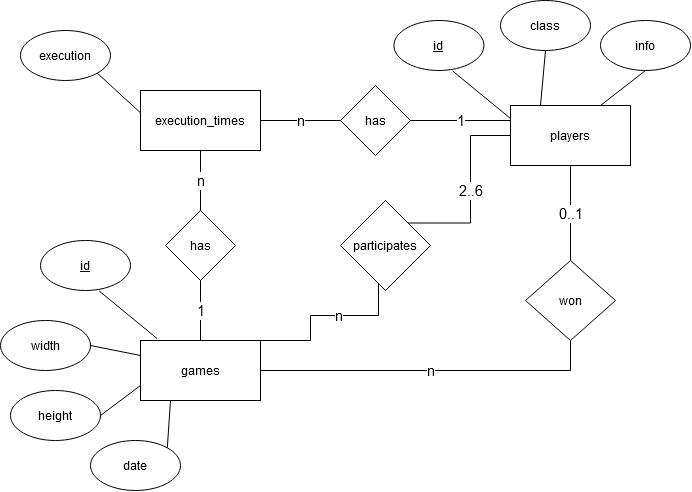
\includegraphics[width=0.9\textwidth]{Bilder/er-diagram.png}
	\caption{\ac{ER}-Modell der Evaluations-\ac{DB}}
	\label{fig:er-schema}
\end{figure}

\subsection{Überführen des \ac{ER}-Modells in ein relationales \acl{DB}-Modell}
\label{subsec:db-schema}

Das \ac{ER}-Modell wurde anschließend in ein relationales Modell überführt, welches die tatsächlichen Relationen in der
Datenbank darstellt.
Dazu wurden Primärschlüssel festgelegt und über Fremdschlüssel Verknüpfungen zwischen den Relationen hergestellt.
Bei der Modellierung wurde darauf geachtet, die dritte Normalform der \ac{DB}-Normalisierung einzuhalten,
um Anomalien und Redundanzen zu verhindern.
\Vgl{db-normalisierung}
In \Abbildung{fig:relationales-db-schema} ist das entworfene relationale Modell zu sehen.

\begin{figure}[htb]
	\centering
	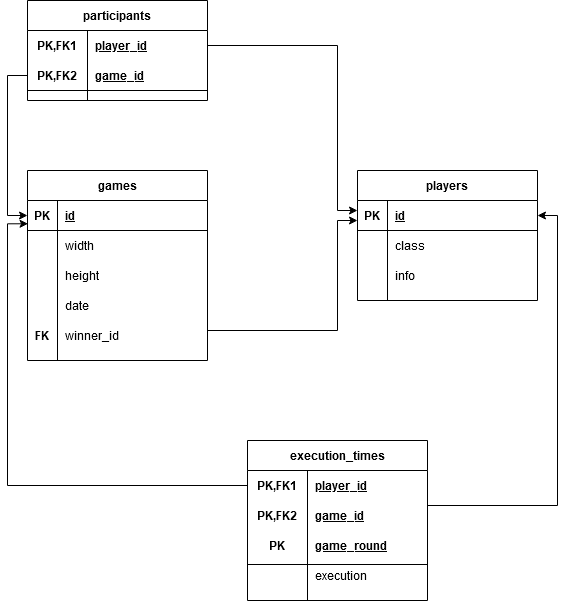
\includegraphics[width=0.5\textwidth]{Bilder/relationales_db_schema.png}
	\caption{Relationales Datenbankschema der Evaluations-Datenbank}
	\label{fig:relationales-db-schema}
\end{figure}

\section{Ergebnis der Evaluation}
\label{sec:ergebnis-evaluation}

Die Evaluation wurde in zwei Etappen durchgeführt.
Für den ersten Teil der Evaluation wurden auf einem Server der Universität Oldenburg insgesamt 1000 Spiele generiert und
insgesamt xx Spielzüge berechnet.
Um aus den in der \ac{DB} gespeicherten Daten die besten \ac{KI}s herauszufiltern, wurde insbesondere jeweils deren
Siegquote in den Spielen betrachtet, bei denen sie teilgenommen haben.
Mit dem in \Anhang{lst:eval-sql-1} abgebildetem SQL-Statement wird eine solche Quote gruppiert nach der \ac{KI}-Klasse
berechnet.

\begin{table}[htb]
    \centering
    \begin{tabular}{|l|c|c|c|c|c|c|c|}
        \hline
		\textbf{Klasse} & {\textbf{Gewonnene Spiele}} & \textbf{Gespielte Spiele} & \textbf{Gewinnrate (\%)} & \textbf{Max Zeit (Sek)} & \textbf{Avg Zeit (Sek)} & \textbf{Avg Zeit oD (Sek)} & \textbf{Deadline eingehalten (\%)} \\ \hline
        NotKillingItselfAI &  &  &  &  &  &  &  \\ \hline
        PathfindingAI &  &  &  &  &  &  &  \\ \hline
		PathfindingSearchTreeAI &  &  &  &  &  &  &  \\ \hline
		SearchTreePathfindingAI &  &  &  &  &  &  &  \\ \hline
		SearchTreeAI &  &  &  &  &  &  &  \\ \hline
		RandomAI &  &  &  &  &  &  &  \\ \hline
    \end{tabular}
    \caption{Steuerung der Oberflächen}
    \label{tab:evaluation-ki-klasse}
\end{table}

\todo{Ergebnis}
Um allerdings ein genaueres Ergebnis zu erhalten, wurde die Abfrage aus \Anhang{lst:eval-sql-2} ausgeführt, welches die
nicht nur die Art der \ac{KI} sondern zusätzlich auch ihre jeweiligen Konfigurations-Parameter betrachtet.

\begin{table}[htb]
    \centering
    \begin{tabular}{|l|c|c|c|c|c|c|c|c|}
        \hline
		\textbf{Klasse} & \textbf{Info} & {\textbf{Gewonnene Spiele}} & \textbf{Gespielte Spiele} & \textbf{Gewinnrate (\%)} & \textbf{Max Zeit (Sek)} & \textbf{Avg Zeit (Sek)} & \textbf{Avg Zeit oD (Sek)} & \textbf{Deadline eingehalten (\%)} \\ \hline
        NotKillingItselfAI &  &  &  &  &  &  &  &  \\ \hline
    \end{tabular}
    \caption{Steuerung der Oberflächen}
    \label{tab:evaluation-ki-konfiguration}
\end{table}

\todo{Ergebnis beschreiben}
Hierbei wird deutlich, dass die \Code{NotKillingItselfAI} deutlich schlechter abschneidet als nach der ersten Auswertung
womöglich angenommen.
Das wird darn liegen, dass die anderen Implementierungen abhängig von der Konfiguration deutlich besser, aber eben auch
deutlich schlechter abschneiden können.

\todo{Kapitel schreiben}
